\section{視線追跡モデルを開発した理由}
近年、AI技術が急速に進化し、画像から様々な情報を取得することが可能になりました。
たとえば、物体検出の分野では、YOLOなどの様々なモデルによって、カメラ画像から人や物体の位置をすばやく検出できるようになっています。
こうした技術を利用し、視線の位置を特定することができれば、視線を利用した新しい操作インターフェースを提供できるのではないかと考えました。

本プロジェクトの目的は、カメラで取得した視線情報をもとに画面上のカーソルを操作するシステムを開発し、ユーザーが手を使わずに目線のみで操作できる新しいインターフェース体験を提供することです。

\section{全体像}
まず初めに、今回開発した「視線で操作するマウスカーソル」のアプリの全体像について説明していきます。

このアプリでは以下の流れによってユーザーの見ている場所にマウスカーソルを動かします。

\begin{algorithm}[H]
    \caption{マウスカーソルを視線位置に動かす流れ}
    \begin{algorithmic}[1]
        \Require PC内蔵カメラ、PC画面サイズ $(W, H)$
        \State \textbf{初期化}: ユーザーにPC画面の4隅(右上、右下、左下、左上)を順に見てもらい、対応する顔画像 $T_i , (i = \text{右上, 右下, 左下, 左上})$ を取得
        \State 顔画像 $T_i$ をもとに、モデルがPC画面上の視線座標 $(x_i, y_i)$ を推定
        \State 視線座標 $(x_i, y_i)$ とPC画面サイズ $(W, H)$ を用いて、射影変換行列 $W$ を作成
        \While{アプリケーションが動作中}
        \State カメラから取得した現在の顔画像をもとに視線座標を推定
        \State 射影変換行列 $W$ を適用して、PC画面上でのユーザーの視線座標を計算
        \State 計算した座標にマウスカーソルを移動
        \EndWhile
    \end{algorithmic}
\end{algorithm}

射影変換行列 $W$ は、モデルが推定したPC画面の4隅の座標に基づく「推定されたPC画面の概形」を「実際のPC画面の概形」に変換するための行列です。

図\ref{fig:coordinate} に、画面の4隅を見ているときの視線推定位置と変換後(画面サイズ)の関係を示します。  
青い点がモデルによって推定された視線位置を表し、赤い正方形がPC画面の領域を表しています。

このとき、青い点(推定された視線位置)を赤い正方形(PC画面の座標系)に変換するためには、射影変換行列 $W$ が必要となります。  
4隅分の視線位置を結ぶ四角形は、必ずしも正方形になるとは限りません。  
そのため、推定された座標系をPC画面の座標系に正確に対応させるために射影変換が必要です。

\begin{figure}[htbp]
    \centering
    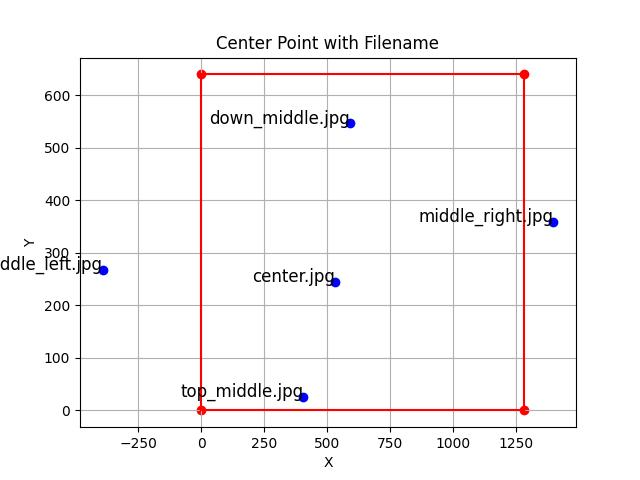
\includegraphics[width=0.7\textwidth]{eye-track-cursor/fig/coordinate.png}
    \caption{視線推定位置(青い点)とPC画面(赤い正方形)の関係}
    \label{fig:coordinate}
\end{figure}

また、本モデルによる顔画像からのPC上で見ている座標の推定の流れは以下の通りです。

\paragraph{モデルの推論の流れ}
\begin{enumerate}
    \item 目の位置を推定
    \item 視線の角度を推定
    \item 1.と2.で取得した「視線の角度・目の位置」をもとに、PC上で見ている箇所を計算
\end{enumerate}

以降では、この「目の位置の推定」と「視線の角度の推定」を行う具体的な方法、そして最終的なアプリによる視線の推定結果について説明していきたいと思います。

\section{目の位置の推定}\label{sec:eye-position}
このモデルは、顔画像から目の位置を推定する際に、PnP(Perspective-n-Point)問題として扱います。PnP問題では、以下の情報をもとにカメラの位置と回転方向を推定します:

\begin{itemize}
    \item カメラの内部パラメータ(焦点距離や歪み係数など)
    \item 画像上の物体の位置と、物体が存在する座標系 $D_{world}$(カメラ基準の座標系 $D_{camera}$ とは異なる基準座標系)における対応関係
\end{itemize}

本モデルでは、これを活用して、顔画像から目の3次元位置を推定します。

\begin{figure}[htbp]
    \centering
    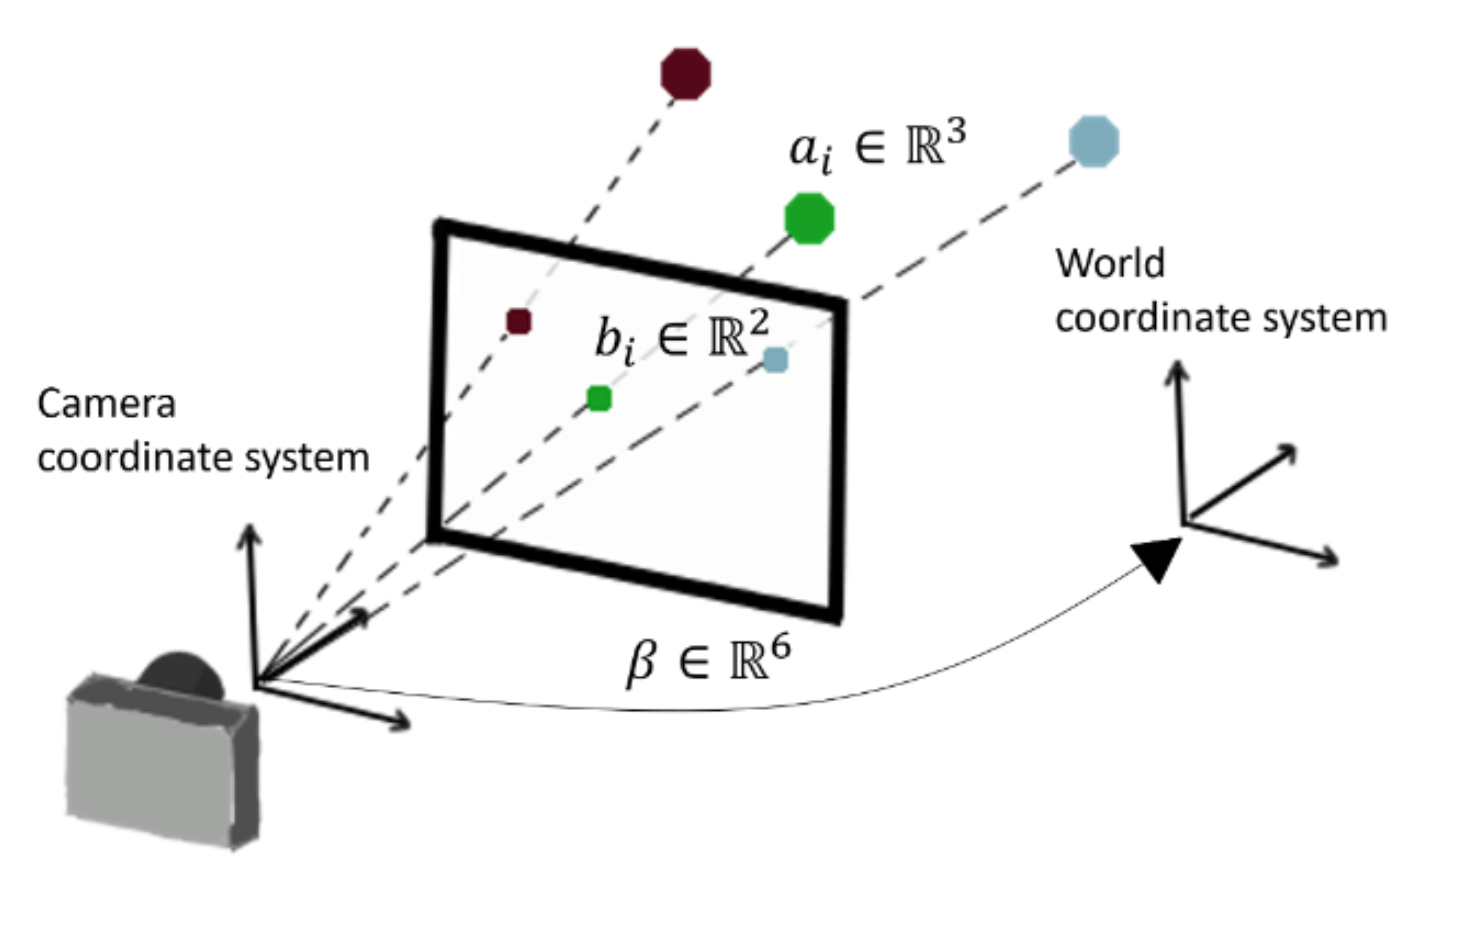
\includegraphics[width=0.7\textwidth]{eye-track-cursor/fig/camera_world_coordinate.png}
    \caption{Camera coordinate system($D_{camera}$)とWorld coordinate system($D_{world}$)の関係性}
    \label{fig:camera_world_coordinate}
\end{figure}

\begin{figure}[htbp]
    \centering
    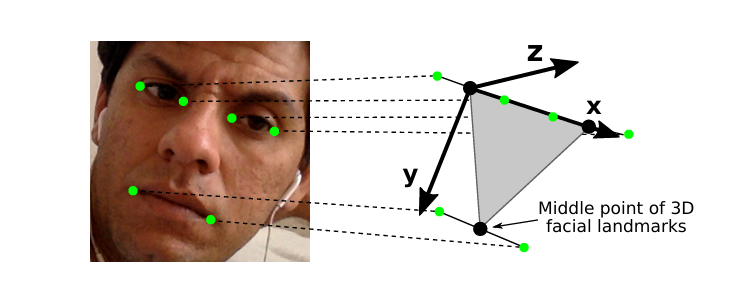
\includegraphics[width=0.7\textwidth]{eye-track-cursor/fig/world_coordinate.png}
    \caption{World coordinate system($D_{world}$)上における顔の特徴点}
    \label{fig:world_coordinate}
\end{figure}

また、顔画像から目の位置を求める流れは以下の通りで、\cite{zhang2017mpiigaze}をもとに作成しました。

\paragraph{目の位置を推定する流れ}
\begin{enumerate}
    \item dlib\footnote{dlibは顔のランドマーク(鼻の位置や目の位置など)を検出するためのライブラリで、今回はERTベースのモデル\cite{valle2018deeply}を使用しています。}を使用して、画像上の顔の特徴的な部分(目や鼻など)を検出
    \item 「カメラの情報(実際のカメラの位置やカメラの焦点距離・歪み係数)」と「1.で検出した特徴点と$D_{world}$上での一般的な顔における関係性」をもとに、\texttt{cv2.solvepnp}を使用してカメラの$D_{world}$上での位置と向き取得
    \item 「1.で求めた画像上での目の場所」と「2.で求めた$D_{world}$上でのカメラの位置と向きから考えられる$D_{camera}$上での頭の位置と向き」を元に、$D_{camera}$上での目の座標を取得
\end{enumerate}

\section{視線の角度推定}
次に、視線の角度を推定するモデルの開発を行いました。このモデル開発においては複数の手法を試しましたので、それらを1つずつ説明していきます。

\subsection{視線の角度推定(手法1)}\label{subsec:gaze-estimation-1}
手法1においては、\cite{zhang2017mpiigaze}にて紹介された視線の角度推定モデルを用い、応用しました。
推定の流れは以下の通りです。

\paragraph{視線の角度を推定する流れ}
\begin{enumerate}
    \item $\blacksquare$\textbf{目の位置を推定する流れ}(\ref{sec:eye-position}節)の2.から、顔の向き $R$ とカメラの位置を取得
    \item \texttt{cv2.warpPerspective}で $R$ とカメラの位置に基づき、$D_{world}$上での目の画像(60×36)を生成
    \item 生成した画像をモデルに入力し、視線角度 $S$ を推定
    \item $S$ と $R$ をもとに、実際のカメラから見た視線情報を算出
\end{enumerate}

また、上記の3.における視線角度推定モデルの構造と学習データセットは以下の通りです。

\paragraph{モデルの構造}
\begin{itemize}
    \item 1層目:EfficientNet(b0)\footnote{最初の層はconv2d(出力チャンネル数:32・カーネルサイズ:3・ストライド:2)に変更しました。}
    \item 2層目:Conv2d
    \item 3層目:Linear+ReLU+Dropout
    \item 4層目:出力値に $R$ を結合
    \item 5層目:Linear+ReLU+Dropout+Linear
\end{itemize}

\paragraph{学習用データ}
\begin{itemize}
    \item MpiiGaze(片目の画像(60×36)と視線情報・顔の向き情報を含むデータセット)
\end{itemize}

論文\cite{zhang2017mpiigaze}では、EfficientNetではなくVGG-16を用いておりました。
しかし、VGG-16よりもEfficientNetの方が計算量が小さく、一般的な画像認識タスクにおける精度も上回っていることから、EfficientNetを採用しました。
このモデルによって、顔の向き(yaw,pitch)を用いて視線方向を実用可能な時間(0.04秒/枚)で推論できました。
yawとpitchの定義は図\ref{fig:yaw_pitch_measurement}に示されているとおりです。

最適化手法としてAdamを使用し、学習率スケジューラーはStepLRを採用しました。

\begin{figure}[htbp]
    \centering
    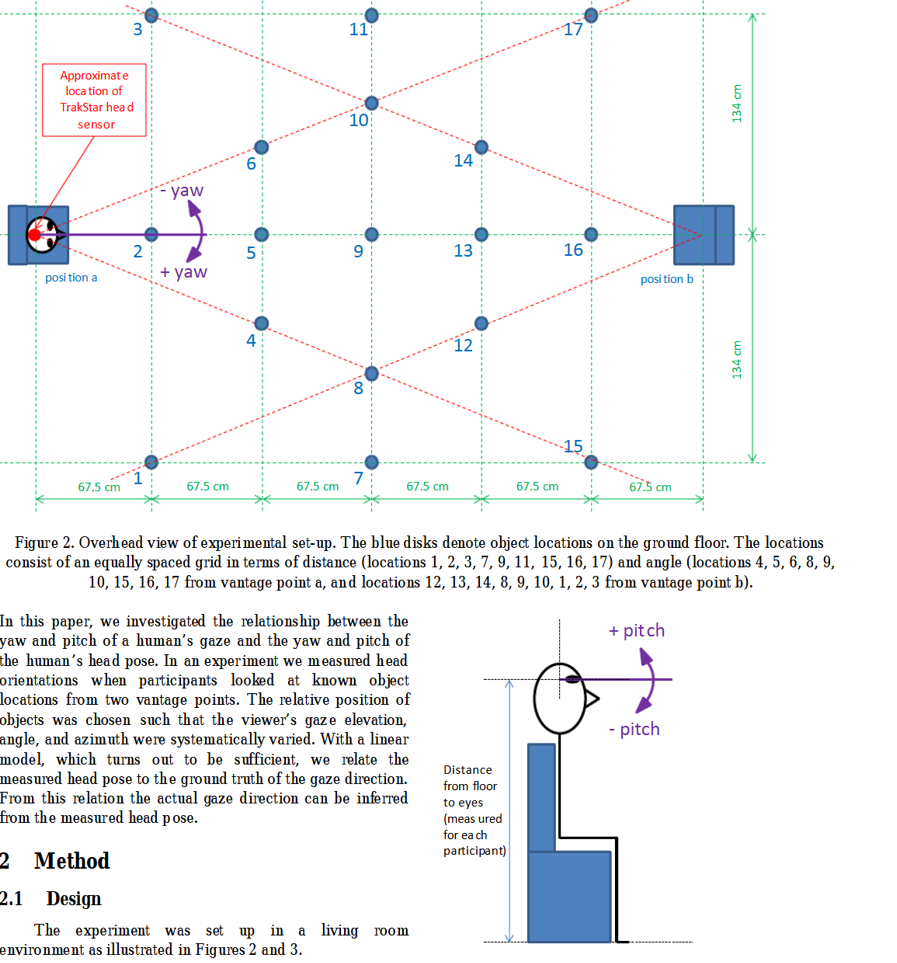
\includegraphics[width=0.7\textwidth]{eye-track-cursor/fig/gaze_definition.png}
    \caption{yawとpitchの定義}
    \label{fig:yaw_pitch_measurement}
\end{figure}

しかし、結果は失敗に終わってしまいました。考えられる原因とその根拠は以下の通りです。

\paragraph{考えられる原因と根拠}
\begin{itemize}
    \item 使用したデータの視線角度範囲が狭く、$\pm 20^\circ$ の範囲に限定されていたため
    \item 訓練時とテスト時の損失値がともに低かったことから、モデルは訓練データの範囲内で良好に動作していることが確認された。しかし、データの視線角度範囲が狭いため、モデルがそれを超える視線角度に対する一般化能力を持てなかった可能性がある。
\end{itemize}

\subsection{視線の角度推定(手法2)}
手法2においては、画像から直接視線の角度を推定する外部モデル(AxGazeEstimation)を活用しました。モデルの推論の流れや実験結果などは以下の通りです。

\paragraph{視線推定モデル(AxGazeEstimation)による推論の流れ}
\begin{enumerate}
    \item BlazeFace\cite{bazarevsky2019blazeface}によって顔とその特徴点(目や鼻など)を検出
    \item 1.にて検出した顔とその特徴点を用いて、ResNetの縮小版(stage3モデル)によって視線角度を推定
\end{enumerate}

\paragraph{結果}
\begin{itemize}
    \item 視線角度の推定に成功しました。(図\ref{fig:gaze_direction_estimation_success})
\end{itemize}

\begin{figure}[htbp]
    \centering
    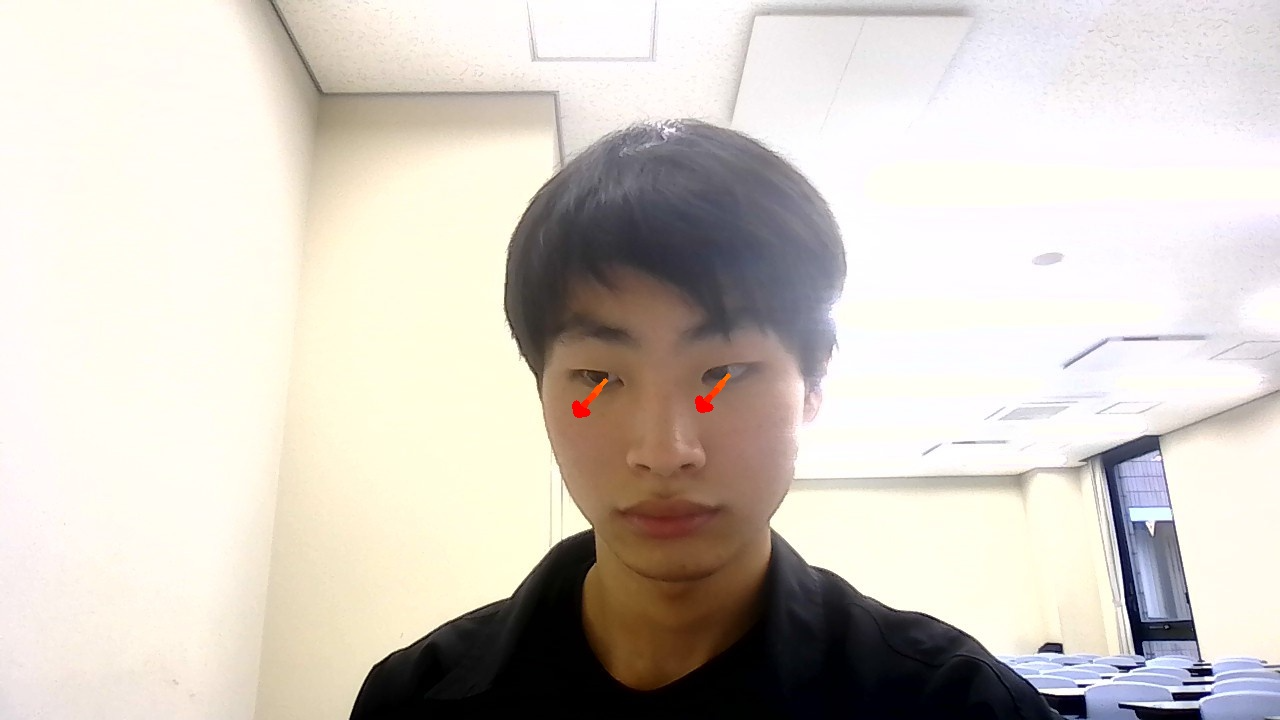
\includegraphics[width=0.7\textwidth]{eye-track-cursor/fig/gaze_direction_result.png}
    \caption{視線角度推定の結果}
    \label{fig:gaze_direction_estimation_success}
\end{figure}

この結果から、視線の角度推定では手法2を採用することにいたしました。

\section{最終結果}
図\ref{fig:gaze_estimation_success}に、視線角度推定の最終結果を示します。
図中の\texttt{middle\_left.jpg}・\texttt{down\_middle.jpg}・\texttt{middle\_right.jpg}・\texttt{top\_middle.jpg}は、
それぞれ画面の左中央・下中央・右中央・上中央
\footnote{画面上の$x$座標・$y$座標におけるPCとの関係は図\ref{fig:definition_coordinates}に示されている通りです。}
を見ている状態に対応しており、概ね正確に推定できていることが確認できます。

\begin{figure}[htbp]
    \centering
    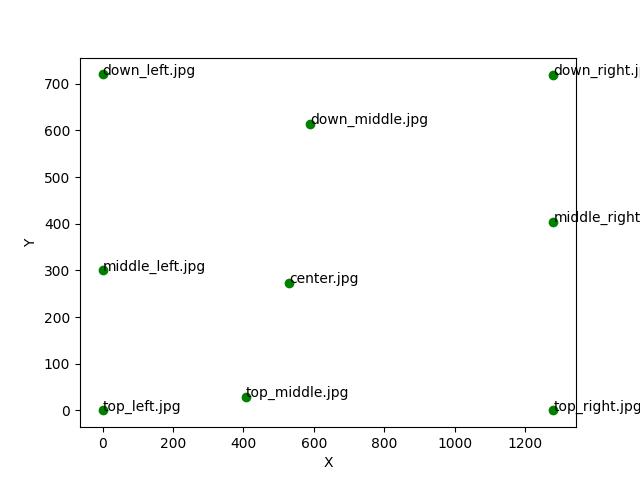
\includegraphics[width=0.7\textwidth]{eye-track-cursor/fig/gaze_at_result.png}
    \caption{視線角度推定の最終結果}
    \label{fig:gaze_estimation_success}
\end{figure}

\begin{figure}[htbp]
    \centering
    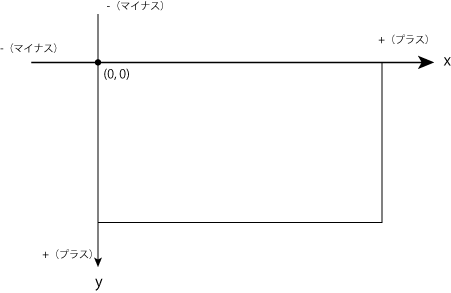
\includegraphics[width=0.7\textwidth]{eye-track-cursor/fig/pc_definition.png}
    \caption{PC上のスクリーン座標系 ($x$: 0~1280, $y$: 0~720)}
    \label{fig:definition_coordinates}
\end{figure}

\section{最後に}
最終的にモデルを作成できましたが、\ref{subsec:gaze-estimation-1}節で述べた手法では十分な性能を達成できませんでした。
この原因として、学習データに問題がある可能性を考えています。
この結果から、モデル構築だけでなく、学習に用いるデータの選定がモデル性能向上において極めて重要であることが分かりました。

他にも、yawとpitchを推定するための様々なモデルや、値の範囲が広い学習データもありましたが、いずれもデータサイズが大きく、ダウンロードしにくい状況でした。
そのため、今後はモデルの改良だけでなく、適切なデータ選定についても学ぶ必要があることが分かりました。

また、今後はデータのyawやpitchの範囲が$-20^\circ \sim 20^\circ$と狭いことが影響している可能性があるため、yawやpitchが$\pm 20^\circ$に近い角度のデータの比重を高め、モデルが広範囲の視線角度に対しても正確に推定できるようにして実験したいです。

\begin{figure}[htbp]
    \centering
    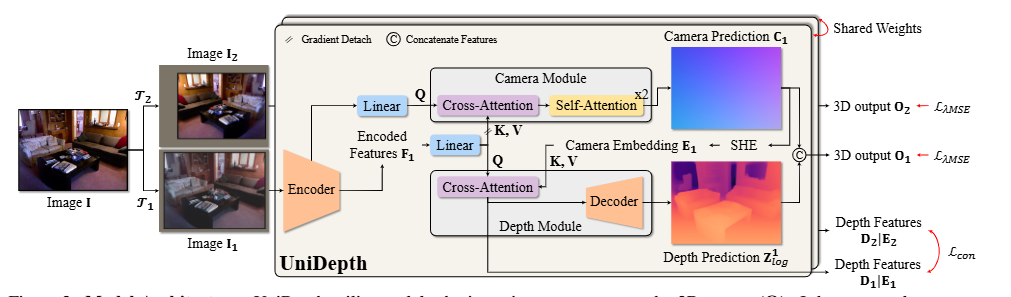
\includegraphics[width=0.7\textwidth]{eye-track-cursor/fig/UniDepth.png}
    \caption{UniDepthの構造 \cite{piccinelli2024unidepthuniversalmonocularmetric}}
    \label{fig:UniDepth}
\end{figure}

また、深度推定においては、UniDepth(図\ref{fig:UniDepth}, \cite{piccinelli2024unidepthuniversalmonocularmetric})などの様々な深度推定モデルが存在します。
こういったモデルを活用することで、目とカメラの距離を推定し、それをもとに目とカメラの正確な位置関係を求めるようにしていきたいです。
